\documentclass[11pt]{article}

\usepackage[margin=1in]{geometry}
\usepackage{amsmath,amssymb,amsthm,mathtools}
\usepackage{booktabs,tabularx,array}
\usepackage{graphicx}
\usepackage{caption}
\usepackage{float}
\usepackage{enumitem}
\usepackage{xcolor}
\usepackage{hyperref}
\usepackage[round]{natbib}
\usepackage{microtype}

\graphicspath{{figures/}}
\hypersetup{colorlinks=true,linkcolor=blue!50!black,citecolor=blue!50!black,urlcolor=blue!50!black}
\setlength{\parindent}{0em}
\setlength{\parskip}{0.45em}
\setlist[itemize]{leftmargin=1.3em,itemsep=0.12em,topsep=0.12em}
\setlist[enumerate]{leftmargin=1.45em,itemsep=0.12em,topsep=0.12em}
\setlength{\emergencystretch}{3em}
\allowdisplaybreaks

\newtheorem{proposition}{Proposition}
\newtheorem{corollary}{Corollary}
\newtheorem{definition}{Definition}
\newtheorem{remark}{Remark}
\newtheorem{assumption}{Assumption}

\newcommand{\dd}{\mathrm d}
\newcommand{\E}{\mathbb E}
\newcommand{\1}{\mathbf 1}
\newcommand{\KK}{\mathcal K}
\newcommand{\HH}{\mathcal H}
\newcommand{\LL}{\mathcal L}

\title{Intergenerational Housing Misallocation and Fertility\\[-0.15em]
\large Compact Theory and Quantitative OLG Blueprint, without Space}
\author{Draft note}
\date{June 9, 2026}

\begin{document}
\maketitle

\begin{abstract}
This note develops a non-spatial theory of intergenerational housing mismatch and fertility. Part I presents a compact analytical model with two overlapping generations. Young households decide whether to enter the housing market and, conditional on entry, choose consumption, housing, and fertility. Old households choose consumption, housing, and bequests. Housing is costly to produce, and policy or contract terms can affect the private cost of holding housing. The model defines a competitive equilibrium and a constrained planner, then compares their marginal allocation rules. Part II gives a quantitative OLG blueprint with many ages, stochastic income, tenure and house-size choice, mortgages, estate taxation, bequest transmission, sequential fertility, and construction of family-capable housing. The quantitative block is a model specification and calibration scaffold, not a results section.
\end{abstract}

\textbf{Overview.} The compact model first describes the economy and the household problems, then defines equilibrium and the planner's problem. The efficiency result is local and conditional on entry: after the competitive and planner allocation rules are defined, the draft compares the true marginal value of housing for already-entered young households and old households. Old occupancy is not inefficient by itself. The relevant gap arises only when young households value housing above its market user cost because access constraints bind, when old households face policy or contract terms that lower the private cost of retaining housing, or both.

\begin{remark}[Status]
The analytical core is closed-form where possible. The quantitative section is intentionally a blueprint. To become a quantitative paper section it needs a parameter vector, data moments, model fit, transition paths, and counterfactual fertility and welfare numbers.
\end{remark}

\clearpage
\tableofcontents
\clearpage

% ==========================================================
\part{Compact Analytical Model}
% ==========================================================

\section{Environment}

The economy is populated by two overlapping generations of households, young and old. Young households are potential parents. They choose whether to enter the modeled housing market; conditional on entry, they choose consumption, housing, and fertility. Old households are incumbent homeowners. They are no longer fertile and choose how much housing to retain, how much to consume, and how much to leave as bequests.

There is one consumption good and one housing service. Housing has flow user cost $q$ and asset price $P$. The two are linked by
\begin{equation}
P=\frac{q}{\rho_p},
\qquad
\rho_p=r+\delta+\tau^p,
\label{eq:compact_price}
\end{equation}
where $r$ is the interest rate, $\delta$ is depreciation, and $\tau^p$ is a recurring property tax. For a given user cost $q$, a higher $\tau^p$ lowers the asset price and hence lowers the down payment required to buy a given amount of housing.

Aggregate housing services are denoted by $H$. They are produced at convex resource cost
\begin{equation}
C(H;Z),
\qquad
C_H(H;Z)>0,
\qquad
C_{HH}(H;Z)>0,
\label{eq:compact_cost}
\end{equation}
where $Z$ is an exogenous shifter of housing supply, interpreted as easier construction or less restrictive land use. Competitive construction implies
\begin{equation}
q=C_H(H;Z).
\label{eq:compact_supply_foc}
\end{equation}
The fixed-stock economy is the limiting case in which the supply schedule is perfectly inelastic.

Let
\begin{equation}
x=1-\tau^b
\end{equation}
denote the after-tax bequest share. The rule assigning estate-tax revenue or rebates is part of fiscal policy.

\section{Young households}

There is a mass $\bar M>0$ of potential young households. A potential young household has type
\[
i=(y_i,a_i,B_i),
\]
drawn from $G_Y$. Here $y_i>0$ is income, $a_i\ge0$ is liquid wealth, and $B_i\ge0$ is gross inheritance exposure. Effective liquid wealth is
\begin{equation}
A_i(x)=a_i+xB_i+T_i^b(x),
\label{eq:compact_liquid_wealth}
\end{equation}
where $T_i^b(x)$ is the estate-tax rebate or transfer assigned to type $i$.

Conditional on entry, young household $i$ chooses consumption $c_i$, housing $h_i$, and fertility $n_i>0$. Children require housing services. Let
\begin{equation}
s_i=h_i-\kappa n_i>0,
\end{equation}
where $\kappa>0$ is the housing requirement per child. Preferences are
\begin{equation}
u_i^Y(c_i,h_i,n_i)
=
\log c_i+\alpha\log(h_i-\kappa n_i)+\beta\log n_i,
\qquad
\alpha,\beta>0.
\label{eq:compact_young_utility}
\end{equation}
The non-housing cost per child is
\begin{equation}
\chi_i=\chi_0+\xi y_i,
\qquad
\chi_0>0,
\qquad
\xi\ge0.
\label{eq:compact_child_cost}
\end{equation}

Given prices and policy, an entered young household solves
\begin{equation}
W_i^Y(q,\tau^p,x)
=
\max_{c_i,h_i,n_i}
\left\{
\log c_i+\alpha\log(h_i-\kappa n_i)+\beta\log n_i
\right\}
\label{eq:compact_young_problem}
\end{equation}
subject to
\begin{align}
c_i+qh_i+\chi_i n_i&=y_i,
\label{eq:compact_young_budget}\\
(1-\phi)Ph_i&\le A_i(x),
\qquad
\phi\in(0,1),
\label{eq:compact_dp}\\
qh_i&\le \psi y_i,
\qquad
\psi\in(0,1).
\label{eq:compact_pti}
\end{align}
Using $P=q/\rho_p$, the two housing-access constraints imply
\begin{equation}
h_i\le
\bar h_i(q,\tau^p,x)
=
\min\left\{
\frac{A_i(x)\rho_p}{(1-\phi)q},
\frac{\psi y_i}{q}
\right\}.
\label{eq:compact_accessible_housing}
\end{equation}

Conditional on entry, this is the only household problem that determines housing and fertility. The outside option enters through the entry decision below.

\section{Old households}

Old households are indexed by $j$ and distributed according to $F_O$. An old household has income $m_j>0$, initial housing $H_j^0$, and a warm-glow bequest utility function $\mathcal B_j$, possibly equal to zero.

Old household $j$ chooses consumption $c_j^O$, retained housing $h_j^O$, and bequest expenditure $e_j\ge0$. Preferences are
\begin{equation}
u_j^O(c_j^O,h_j^O,e_j)
=
\log c_j^O+\gamma\log h_j^O+\mathcal B_j(e_j),
\qquad
\gamma>0.
\label{eq:compact_old_utility}
\end{equation}

The household owns $H_j^0$ units of housing. It faces policy or contract terms that make retaining housing privately attractive. The compact budget writes these terms directly as a reduction in the private cost of retained housing:
\begin{equation}
c_j^O+e_j+
\left[q-\ell_j-\omega_j^p xq\right]h_j^O
=
m_j+qH_j^0,
\qquad
0\le h_j^O\le H_j^0.
\label{eq:compact_old_budget}
\end{equation}
Assume
\begin{equation}
0\le \ell_j+\omega_j^p xq<q.
\label{eq:compact_old_private_cost_positive}
\end{equation}

The terms $\ell_j$ and $\omega_j^p xq$ are not preferences. They represent policy or contract terms, such as a tax-basis advantage, a retention subsidy, or a mortgage-contract benefit. If these terms have fiscal, lender, or administrative resource costs, those costs appear in the aggregate resource constraint. True housing utility and true warm-glow bequest utility are already in $u_j^O$ and are counted by the planner.

\section{Entry}

A potential young household can enter the modeled housing market or take an outside option. The outside value is $\bar W^E$. Entry is subject to Type-I extreme-value taste shocks with scale $\kappa_E>0$. The probability that type $i$ enters is
\begin{equation}
\pi_i^E(q,\tau^p,x)
=
\frac{
\exp\{W_i^Y(q,\tau^p,x)/\kappa_E\}
}{
\exp\{W_i^Y(q,\tau^p,x)/\kappa_E\}
+
\exp\{\bar W^E/\kappa_E\}
}.
\label{eq:compact_entry_prob}
\end{equation}
The endogenous measure of young entrants is
\begin{equation}
\dd F_Y^E(i;q,\tau^p,x)
=
\bar M\,\pi_i^E(q,\tau^p,x)\,\dd G_Y(i).
\label{eq:compact_entry_measure}
\end{equation}
The limit $\kappa_E\downarrow0$ gives deterministic entry. Conditional on entry, the household first-order conditions are those of \eqref{eq:compact_young_problem}.

\section{Competitive equilibrium}

Given policies $(\tau^p,x,Z)$, transfer rule $T_i^b(x)$, and old policy or contract terms $(\ell_j,\omega_j^p)$, aggregate housing demand is
\begin{equation}
H^D(q;\tau^p,x)
=
\bar M
\int
\pi_i^E(q,\tau^p,x)
h_i^Y(q,\tau^p,x)
\,\dd G_Y(i)
+
\int h_j^O(q,x)\,\dd F_O(j).
\label{eq:compact_hd}
\end{equation}

\begin{definition}[Competitive equilibrium]
Given $(\tau^p,x,Z)$, a competitive equilibrium consists of a user cost $q$, an asset price $P$, young allocations $\{c_i,h_i,n_i\}$, entry probabilities $\{\pi_i^E\}$, old allocations $\{c_j^O,h_j^O,e_j\}$, and aggregate housing $H$ such that:
\begin{enumerate}
\item conditional on entry, young households solve \eqref{eq:compact_young_problem};
\item old households solve \eqref{eq:compact_old_budget};
\item entry is given by \eqref{eq:compact_entry_prob};
\item $P=q/\rho_p$;
\item competitive construction satisfies $q=C_H(H;Z)$, with the fixed-stock case obtained by taking $H$ as exogenous;
\item fiscal, lender, or tax-expenditure accounts associated with $T_i^b(x)$, $\ell_j$, and $\omega_j^p$ are closed;
\item the housing market clears:
\begin{equation}
H^D(q;\tau^p,x)=H.
\label{eq:compact_clearing}
\end{equation}
\end{enumerate}
\end{definition}

Aggregate fertility is
\begin{equation}
N(q;\tau^p,x)
=
\bar M
\int
\pi_i^E(q,\tau^p,x)n_i(q,\tau^p,x)
\,\dd G_Y(i).
\label{eq:compact_aggregate_fertility}
\end{equation}

\section{Constrained planner}

The planner has the same preferences, type distributions, entry technology, and housing technology as the competitive economy. The planner chooses entry-relevant inside allocations, young consumption, housing and fertility, old consumption, housing and bequests, and aggregate housing. The planner can use lump-sum transfers of the consumption good. The planner respects aggregate resources and the housing technology.

The planner counts true old housing utility and true warm-glow bequest utility. It does not count the private cost reductions in \eqref{eq:compact_old_budget} as utility or as resource savings. If those terms require real resources, their cost is included below.

Let $\omega_i^Y>0$ and $\omega_j^O>0$ be Pareto weights. Let $\mathcal G_i(n_i)$ denote an optional social payoff from births beyond parental utility. The fertility-neutral planner has $\mathcal G_i\equiv0$.

If the planner assigns young type $i$ conditional allocation $(c_i,h_i,n_i)$, the inside value relevant for entry is
\begin{equation}
V_i^P=u_i^Y(c_i,h_i,n_i).
\label{eq:compact_planner_inside_value}
\end{equation}
The induced entry probability is
\begin{equation}
\pi_i^P
=
\frac{
\exp\{V_i^P/\kappa_E\}
}{
\exp\{V_i^P/\kappa_E\}
+
\exp\{\bar W^E/\kappa_E\}
}.
\label{eq:compact_planner_entry_prob}
\end{equation}
The corresponding expected entry value, up to an additive constant, is
\begin{equation}
\mathcal W_i^E(V_i^P)
=
\kappa_E
\log
\left[
\exp\{V_i^P/\kappa_E\}
+
\exp\{\bar W^E/\kappa_E\}
\right].
\label{eq:compact_entry_logsum}
\end{equation}

The planner solves
\begin{equation}
\max
\left\{
\bar M\int
\omega_i^Y\mathcal W_i^E(V_i^P)\,\dd G_Y(i)
+
\bar M\int
\pi_i^P\mathcal G_i(n_i)\,\dd G_Y(i)
+
\int
\omega_j^O u_j^O(c_j^O,h_j^O,e_j)\,\dd F_O(j)
\right\}
\label{eq:compact_planner_problem}
\end{equation}
subject to
\begin{align}
\bar M\int \pi_i^P h_i\,\dd G_Y(i)
+
\int h_j^O\,\dd F_O(j)
&\le H,
\label{eq:compact_planner_housing}\\
\bar M\int
\pi_i^P(c_i+\chi_i n_i-y_i)\,\dd G_Y(i)
+
\int(c_j^O+e_j-m_j)\,\dd F_O(j)
+
C(H;Z)+\Xi^\Pi
&\le0.
\label{eq:compact_planner_goods}
\end{align}
Here $\Xi^\Pi\ge0$ is the real resource cost of the policy environment. If the policy or contract terms in \eqref{eq:compact_old_budget} are pure transfers among households, taxpayers, and lenders, then $\Xi^\Pi=0$.

The planner problem has two margins. The first is the entry margin. The second is the conditional allocation margin among households who enter. The local efficiency result below concerns the second margin: it compares the value of housing for an already-entered young household and an old household, holding entry probabilities fixed at the instant of the reassignment.

Let $\Lambda$ be the multiplier on goods feasibility and let $\Lambda Q$ be the multiplier on housing feasibility. Conditional on entry probabilities, an interior planner allocation satisfies
\begin{align}
\frac{u^Y_{h,i}}{u^Y_{c,i}}&=Q,
\label{eq:compact_planner_young_housing}\\
\frac{u^O_{h,j}}{u^O_{c,j}}&=Q,
\label{eq:compact_planner_old_housing}\\
Q&=C_H(H;Z),
\label{eq:compact_planner_supply}\\
\frac{\beta c_i}{n_i}+\nu_i^g&=\chi_i+\kappa Q,
\label{eq:compact_planner_fertility}\\
\frac{\mathcal B_j'(e_j)}{u^O_{c,j}}&=1
\qquad \text{if }e_j>0.
\label{eq:compact_planner_bequest}
\end{align}
The term $\nu_i^g$ is the goods-equivalent social value of a marginal birth beyond parental utility. If $\mathcal G_i\equiv0$, then $\nu_i^g=0$.

\section{Marginal conditions in equilibrium}

The household optimality conditions imply two marginal wedges relative to the planner's allocation rules.

For young household $i$, let $\lambda_i$ be the multiplier on \eqref{eq:compact_young_budget}, $\mu_i$ the multiplier on \eqref{eq:compact_dp}, and $\eta_i$ the multiplier on \eqref{eq:compact_pti}. At an interior allocation,
\begin{align}
\frac{1}{c_i}&=\lambda_i,
\label{eq:compact_young_foc_c}\\
\frac{\alpha}{h_i-\kappa n_i}
&=
\lambda_i q+\mu_i(1-\phi)P+\eta_i q,
\label{eq:compact_young_foc_h}\\
\frac{\beta}{n_i}
&=
\lambda_i\chi_i+
\frac{\alpha\kappa}{h_i-\kappa n_i}.
\label{eq:compact_young_foc_n}
\end{align}
Define the goods-equivalent young housing shadow value by
\begin{equation}
\zeta_i
=
\frac{\mu_i}{\lambda_i}(1-\phi)P
+
\frac{\eta_i}{\lambda_i}q
\ge0.
\label{eq:compact_zeta}
\end{equation}
The young household's true marginal value of housing is
\begin{equation}
MV_i^Y
\equiv
\frac{u^Y_{h,i}}{u^Y_{c,i}}
=
\frac{\alpha c_i}{h_i-\kappa n_i}.
\label{eq:compact_mv_y}
\end{equation}
Combining \eqref{eq:compact_young_foc_h} and \eqref{eq:compact_zeta},
\begin{equation}
MV_i^Y=q+\zeta_i.
\label{eq:compact_young_wedge}
\end{equation}

For old household $j$, define
\begin{equation}
L_j^p(q,x)=\ell_j+\omega_j^p xq.
\label{eq:compact_Lp}
\end{equation}
This is the private policy or contract wedge implied by \eqref{eq:compact_old_budget}. It is not a preference term. At an interior old allocation,
\begin{equation}
MV_j^O
\equiv
\frac{u^O_{h,j}}{u^O_{c,j}}
=
\frac{\gamma c_j^O}{h_j^O}
=
q-L_j^p(q,x).
\label{eq:compact_old_wedge}
\end{equation}
If bequests are interior, then
\begin{equation}
\mathcal B_j'(e_j)=\frac{1}{c_j^O}.
\label{eq:compact_old_bequest_foc}
\end{equation}
This is a true preference margin, not a wedge.

The young fertility condition follows from \eqref{eq:compact_young_foc_n}. Multiplying by $c_i=1/\lambda_i$ and using \eqref{eq:compact_young_wedge} gives
\begin{equation}
\frac{\beta c_i}{n_i}
=
\chi_i+\kappa(q+\zeta_i).
\label{eq:compact_fertility_wedge}
\end{equation}
Thus a binding housing-access constraint raises the effective marginal cost of a child by $\kappa\zeta_i$.

If $\zeta_i=0$, define $\mathcal A=1+\alpha+\beta$. The unconstrained young demands are
\begin{align}
c_i^u&=\frac{y_i}{\mathcal A},
&
h_i^u-\kappa n_i^u&=\frac{\alpha y_i}{\mathcal A q},
\label{eq:compact_unconstrained_c_s}\\
n_i^u&=\frac{\beta y_i}{\mathcal A(\chi_i+\kappa q)},
&
h_i^u&=
\frac{\alpha y_i}{\mathcal A q}
+
\kappa
\frac{\beta y_i}{\mathcal A(\chi_i+\kappa q)}.
\label{eq:compact_unconstrained_n_h}
\end{align}
When \eqref{eq:compact_accessible_housing} binds, the household sets $h_i=\bar h_i(q,\tau^p,x)$, and fertility is pinned down by the one-dimensional condition
\begin{equation}
\frac{\beta}{n_i}
=
\frac{\chi_i}{y_i-q\bar h_i-\chi_i n_i}
+
\frac{\alpha\kappa}{\bar h_i-\kappa n_i}.
\label{eq:compact_constrained_fertility}
\end{equation}

\section{Efficiency}

\begin{proposition}[No-wedge benchmark, conditional on entry]
Consider an interior competitive equilibrium. Suppose no young housing-access constraint binds, so $\zeta_i=0$ for all entered young types. Suppose old households face no policy or contract retention term, so $L_j^p(q,x)=0$ for all old types. Suppose $\nu_i^g=0$ and all policy accounts are resource-neutral. Then, conditional on the equilibrium entry measure, the competitive allocation satisfies the planner's conditional housing, fertility, and construction first-order conditions for suitable Pareto weights.
\end{proposition}

\begin{proof}
If $\zeta_i=0$, then \eqref{eq:compact_young_wedge} gives $MV_i^Y=q$ for every entered young type. If $L_j^p(q,x)=0$, then \eqref{eq:compact_old_wedge} gives $MV_j^O=q$ for every interior old type. Competitive construction gives $q=C_H(H;Z)$. Hence
\[
MV_i^Y=MV_j^O=C_H(H;Z),
\]
which is the planner's conditional housing allocation rule with $Q=q$. With $\nu_i^g=0$, \eqref{eq:compact_fertility_wedge} becomes
\[
\frac{\beta c_i}{n_i}=\chi_i+\kappa q,
\]
which is the planner's conditional fertility rule evaluated at $Q=q$. Pareto weights can be chosen to support the competitive consumption allocation. The entry margin determines the mass and composition of young households; it does not alter these conditional first-order conditions.
\end{proof}

The proposition is conditional on entry. It does not say that the competitive entry allocation is globally optimal for arbitrary Pareto weights or arbitrary outside-option welfare weights. It says that, absent the two housing wedges and absent an external fertility value, the conditional allocation of housing, fertility, and construction satisfies the planner's marginal rules.

\begin{proposition}[Young-old housing wedge, conditional on entry]
Fix an interior competitive equilibrium. Consider an already-entered young household $i$ and an old household $j$. Suppose an institution can locally assign an infinitesimal unit of existing housing from $j$ to $i$, hold entry fixed at the instant of reassignment, and use compensating transfers of the consumption good. The direct goods-equivalent surplus from the reassignment is
\begin{equation}
\Delta_{ij}
=
MV_i^Y-MV_j^O
=
\zeta_i+L_j^p(q,x).
\label{eq:compact_local_wedge}
\end{equation}
If $\zeta_i+L_j^p(q,x)>0$, the competitive allocation violates the planner's conditional young-old housing allocation rule on margin $(i,j)$.
\end{proposition}

\begin{proof}
Equations \eqref{eq:compact_young_wedge} and \eqref{eq:compact_old_wedge} imply
\[
MV_i^Y-MV_j^O
=
(q+\zeta_i)-\left[q-L_j^p(q,x)\right]
=
\zeta_i+L_j^p(q,x).
\]
The planner counts true young utility, true old housing utility, and true old bequest utility. The planner does not count $L_j^p(q,x)$ as utility or as a resource saving. Hence the expression above is the direct goods-equivalent surplus from the conditional reassignment.

With a transfer $T$ from young $i$ to old $j$, the young household's first-order gain is $(MV_i^Y-T)\dd\varepsilon$, and the old household's first-order gain is $(T-MV_j^O)\dd\varepsilon$. If $MV_i^Y>MV_j^O$, choose $T\in(MV_j^O,MV_i^Y)$. Both gains are then positive to first order.
\end{proof}

This proposition is the weakened, correct version of the efficiency claim. It is not a claim that a planner can erase private borrowing constraints without instruments. It is a local compensated-reallocation result, or equivalently a shadow-value statement for an institution that can relax the young housing allocation margin.

\section{Fertility and entry}

The same young housing shadow value appears in the fertility condition:
\[
\frac{\beta c_i}{n_i}
=
\chi_i+\kappa q+\kappa\zeta_i.
\]
The term $\kappa\zeta_i$ is an implicit child tax. A marginal child requires $\kappa$ units of housing, and a constrained young household values housing at $q+\zeta_i$, not at the market user cost $q$.

The outside option affects aggregate fertility through entry. For perturbations that change either conditional fertility or entry probabilities,
\begin{equation}
\dd N
=
\bar M
\int
\left[
\pi_i^E\,\dd n_i
+
n_i\,\dd\pi_i^E
\right]\dd G_Y(i).
\label{eq:compact_entry_fertility}
\end{equation}
The first term is the intensive fertility margin among entrants. The second term is the extensive entry margin. Both affect aggregate fertility, but only the first is part of the conditional young-old housing wedge in \eqref{eq:compact_local_wedge}.

Old occupancy is not inefficient by itself. If old housing demand reflects true old housing utility or true warm-glow bequest utility, those motives are part of $u_j^O$ and are counted by the planner. Inefficiency arises when young households face a positive housing-access shadow value, $\zeta_i>0$, when old retention is supported by a policy or contract term, $L_j^p(q,x)>0$, or both.

% ==========================================================
\part{Quantitative OLG Blueprint without Space}
% ==========================================================

\section{Purpose, timing, and state space}

The quantitative block embeds the compact wedge in a finite-life OLG economy with income risk, tenure and house-size choice, mortgages, bequests, sequential fertility, and increasing supply. It remains non-spatial. It is not a results section.

Time is annual. Households live from age $a=1$ to $A$. Survival is $\pi_a$. Fertility is possible for $a\in\mathcal F$. The household chooses a birth indicator
\begin{equation}
f_t\in\{0,1\},\qquad n_{t+1}=n_t+f_t\le\bar n.
\label{eq:birth_indicator_quant}
\end{equation}
Children are tracked by a child-age vector $g_t=(g_{0,t},\ldots,g_{S_c,t})$ with law of motion
\begin{equation}
g_{t+1}=(f_t,g_{0,t},\ldots,g_{S_c-1,t}),
\qquad m(g_t)=\sum_{s=0}^{S_c}g_{s,t}.
\label{eq:child_aging_quant}
\end{equation}
This fixes fertility timing as sequential parity hazards; there is no one-shot completed-fertility jump.

\begin{figure}[H]
\centering
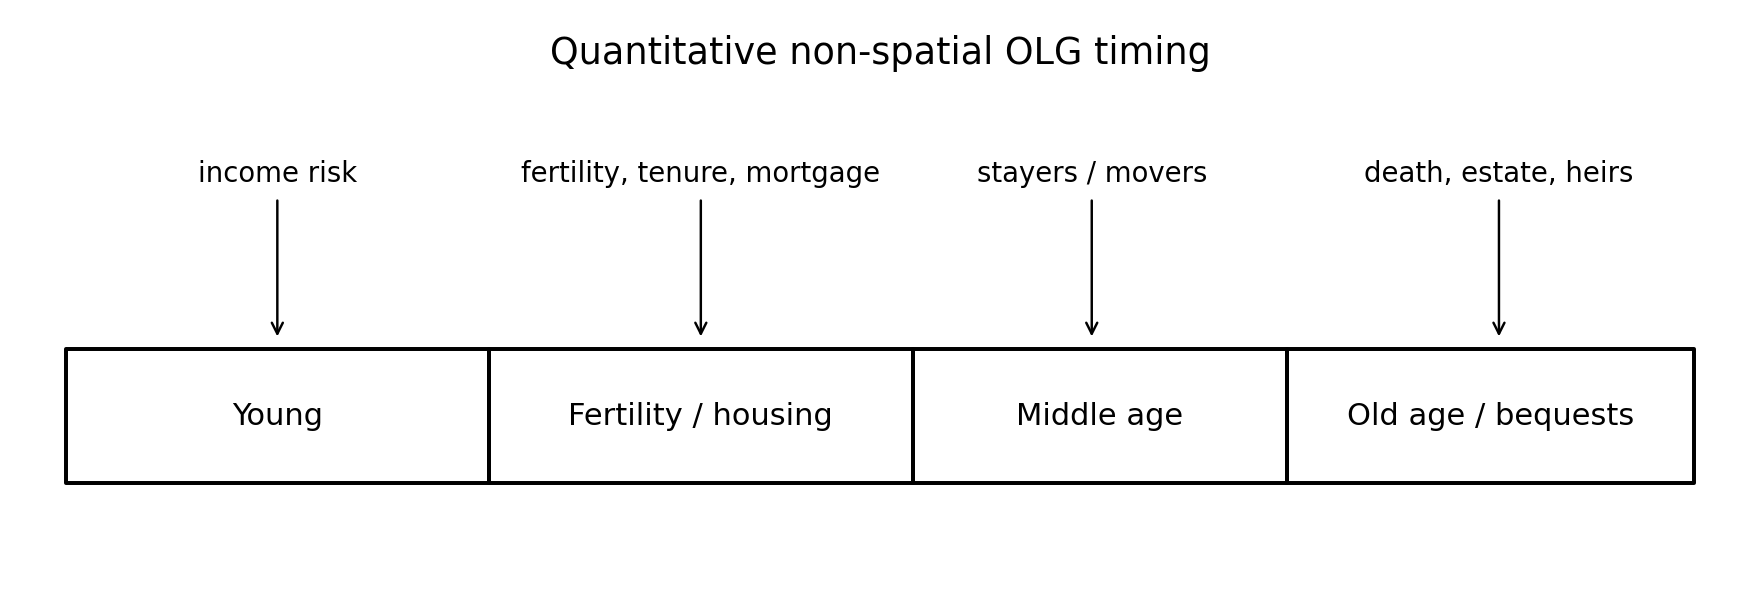
\includegraphics[width=0.90\textwidth]{fig3_olg_timeline.png}
\caption{Quantitative non-spatial OLG timing. Households move through income risk, sequential births, housing adjustment, mortgage choices, aging, death, and bequest transmission.}
\label{fig:olg_timeline}
\end{figure}

The individual state is
\begin{equation}
s_t=(a,z,b,o,k,d,m^d,\iota,n,g,B),
\label{eq:state_quant}
\end{equation}
where $a$ is age, $z$ is idiosyncratic productivity, $b$ is liquid assets, $o\in\{R,O\}$ is tenure, $k\in\KK$ is occupied housing size, $d$ is mortgage debt, $m^d$ is remaining mortgage maturity, $\iota$ is the incumbent coupon, $n$ is completed fertility, $g$ is the child-age vector, and $B$ is inherited liquid wealth.

The key convention is
\begin{equation}
\KK=\{S,M,L\}.
\end{equation}
The size $k$ produces housing services for both renters and owners. Tenure $o$ determines whether the household pays rent or owns. Renters have $d=0$, $m^d=0$, and no incumbent coupon, but they still choose $k$ and consume $h_k$ services.

Income is
\begin{equation}
y_t(a,z)=W_t e_a z,
\qquad z'\sim\Pi_z(\cdot\mid z).
\label{eq:income_quant}
\end{equation}

\begin{table}[H]
\centering
\caption{Quantitative state variables and units}
\small
\begin{tabularx}{\textwidth}{@{}lX@{}}
\toprule
Object & Meaning \\
\midrule
$a,z,b$ & Age, idiosyncratic productivity, liquid assets \\
$o\in\{R,O\}$ & Tenure: rent or own \\
$k\in\KK=\{S,M,L\}$ & Occupied housing size for both renters and owners \\
$h_k$ & Service units delivered by one size-$k$ dwelling \\
$d,m^d,\iota$ & Mortgage balance, remaining maturity, incumbent coupon \\
$n,g$ & Completed fertility and child-age vector \\
$B$ & Inherited liquid wealth \\
$P_{k,t}$ & Asset price per service unit of size-$k$ housing \\
$R_{k,t}$ & Rental/user cost per service unit of size-$k$ housing \\
$H_{k,t},I_{k,t}$ & Stock and construction of service units of size $k$ \\
\bottomrule
\end{tabularx}
\end{table}

\section{Preferences and housing services}

Housing slack is
\begin{equation}
\sigma(k,g)=h_k-\kappa m(g).
\end{equation}
Period utility is
\begin{equation}
u(c,k,n,g)=\frac{\left[c^{1-\alpha_h}\sigma(k,g)^{\alpha_h}\right]^{1-\sigma_u}-1}{1-\sigma_u}+\varphi_n v(n),
\label{eq:period_utility_quant}
\end{equation}
with the log limit when $\sigma_u=1$. The non-housing child cost is
\begin{equation}
\chi_t(a,z,g)=\chi_0m(g)+\xi y_t(a,z)m(g).
\label{eq:child_cost_quant}
\end{equation}

\section{Tenure, mortgages, and lock-in}

A renter of size $k'$ pays $R_{k',t}h_{k'}$ and chooses $d'=0$. An owner who buys size $k'$ pays $P_{k',t}h_{k'}$ and can borrow $d'$. Since $P_{k,t}$ is a price per service unit, $P_{k,t}h_k$ is the asset price of a size-$k$ dwelling. New owner mortgages satisfy
\begin{align}
d'&\le \phi P_{k',t}h_{k'},\label{eq:ltv_quant}\\
\mathcal P(d',R_t^m,m_0)&\le \psi y_t(a,z),\label{eq:pti_quant}
\end{align}
where $m_0$ is origination maturity. The fixed annual mortgage payment is
\begin{equation}
\mathcal P(d,R,m)=d\frac{R}{1-(1+R)^{-m}},
\label{eq:mortgage_payment}
\end{equation}
with zero-rate limit $d/m$.

An incumbent owner keeping the same house keeps the old coupon $\iota$. Moving or refinancing replaces it with $R_t^m$. The present-value lock-in cost of losing a below-market coupon is
\begin{equation}
\mathcal L_t^m(d,\iota,m^d;R_t^m)=\max\left\{\sum_{s=1}^{m^d}\frac{\mathcal P(d,R_t^m,m^d)-\mathcal P(d,\iota,m^d)}{(1+r_t)^s},0\right\}.
\label{eq:pv_lockin_quant}
\end{equation}
Adjustment cost is
\begin{equation}
\Phi_t(k,d,m^d,\iota)=\lambda_s P_{k,t}h_k+\mathcal L_t^m(d,\iota,m^d;R_t^m).
\label{eq:adjustment_quant}
\end{equation}
The real resource cost is $\lambda_sP_{k,t}h_k$. The coupon term is a borrower-lender transfer unless mortgage investors are outside the economy.

The budget is written compactly as
\begin{equation}
c+b'+\mathcal X_t(o',k',d',m^{d\prime},\iota'\mid o,k,d,m^d,\iota)+\chi_t(a,z,g')=y_t(a,z)+(1+r_t)b+T_t(s),
\label{eq:budget_quant}
\end{equation}
where $\mathcal X_t$ is evaluated by tenure branch: renters pay rent; owner stayers pay mortgage payments, maintenance, and property taxes; movers sell, repay debt, forfeit the coupon value, pay transaction costs, buy, and choose new debt, maturity, and coupon; sellers liquidate equity and rent.

\section{Bequests, estate taxation, and transfers}

At death, the estate is
\begin{equation}
E_t(s)=\max\{b+\1\{o=O\}(P_{k,t}h_k-d),0\}.
\end{equation}
Estate-tax revenue is
\begin{equation}
\mathcal R_t^b=\tau_t^b\int E_t(s)\,\dd D_t(s),
\label{eq:estate_tax_revenue_quant}
\end{equation}
where $D_t$ is the decedent distribution. After-tax estates are assigned to heirs using a kernel $\Gamma_t(s^h\mid s^d)$:
\begin{equation}
B_{t+1}(s^h)=\int (1-\tau_t^b)E_t(s^d)\Gamma_t(s^h\mid s^d)\,\dd D_t(s^d).
\label{eq:inheritance_kernel_quant}
\end{equation}
A family-linked kernel assigns estates to actual descendants; an anonymous kernel draws heirs from the aggregate estate distribution. Estate-tax revenue is rebated according to $T_t^b(s)$ satisfying
\begin{equation}
\int T_t^b(s)\,\dd\mu_t(s)=\mathcal R_t^b
\label{eq:estate_rebate_quant}
\end{equation}
when the reform is revenue-neutral. A repeal counterfactual must specify both $\Gamma_t$ and $T_t^b$.

Old households may also have true warm-glow bequest utility
\begin{equation}
\mathcal B(E_t)=\theta_B\frac{\left[(1-\tau_t^b)E_t+\underline b\right]^{1-\sigma_B}}{1-\sigma_B}.
\label{eq:warm_glow_quant}
\end{equation}
This is not an inefficiency. The planner counts \eqref{eq:warm_glow_quant}. It is distinct from policy-created retention wedges.

\section{Housing supply and units}

For each size $k\in\KK$, $H_{k,t}$ is measured in service units. A size-$k$ dwelling delivers $h_k$ services. The stock law is
\begin{equation}
H_{k,t+1}=(1-\delta_k)H_{k,t}+I_{k,t},
\label{eq:stock_law_quant}
\end{equation}
where $I_{k,t}$ is construction in service units. Developers have cost
\begin{equation}
C_{k,t}(I)=\frac{\chi_k}{1+\eta_k}\left(\frac{I}{Z_{k,t}}\right)^{1+\eta_k}Z_{k,t},
\qquad \eta_k>0.
\label{eq:construction_quant}
\end{equation}
Competitive construction implies
\begin{equation}
P_{k,t}=C'_{k,t}(I_{k,t})=\chi_k\left(\frac{I_{k,t}}{Z_{k,t}}\right)^{\eta_k}.
\label{eq:developer_foc_quant}
\end{equation}
The rental/user cost satisfies
\begin{equation}
R_{k,t}=(r_t+\delta_k+\tau_t^p)P_{k,t}-\E_t(P_{k,t+1}-P_{k,t}).
\label{eq:user_cost_quant}
\end{equation}

\begin{figure}[H]
\centering
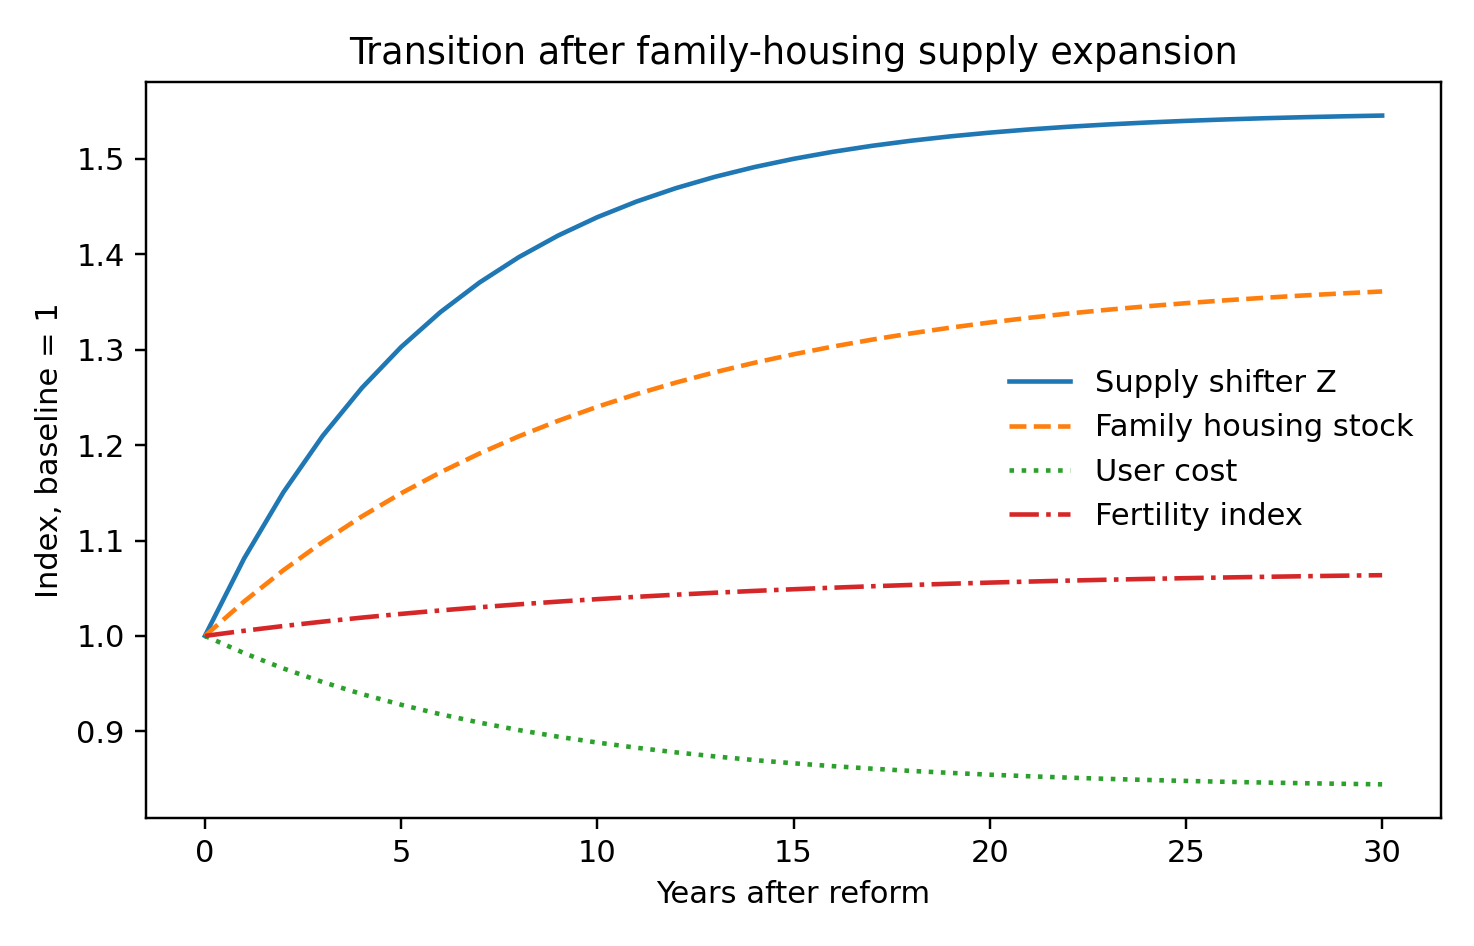
\includegraphics[width=0.82\textwidth]{fig4_supply_transition.png}
\caption{Supply expansion in the quantitative model. A rise in $Z_{M,t}$ or $Z_{L,t}$ increases construction of family-capable housing and reduces user costs along the transition.}
\label{fig:supply_transition}
\end{figure}

\section{Household dynamic program}

Let $V_t(s)$ be the household value. With $n'=n+f_t$ and $g'$ determined by \eqref{eq:child_aging_quant},
\begin{equation}
V_t(s)=\max_{c,b',o',k',d',m^{d\prime},\iota',f_t}\left\{u(c,k',n',g')+\beta\pi_a\E[V_{t+1}(s')\mid s,\text{choices}]+\beta(1-\pi_a)\mathcal B(E_t(s'))\right\}
\label{eq:bellman_quant}
\end{equation}
subject to \eqref{eq:budget_quant}, \eqref{eq:ltv_quant}--\eqref{eq:pti_quant}, income transitions, child aging, tenure feasibility, mortgage amortization, bequest transmission, and nonnegativity constraints. The next state is
\begin{equation}
s'=(a+1,z',b',o',k',d',m^{d\prime},\iota',n',g',B').
\end{equation}

\section{Recursive competitive equilibrium}

Let $\mu_t$ be the distribution over states. A recursive competitive equilibrium is a sequence of prices $\{P_{k,t},R_{k,t},R_t^m,r_t\}$, taxes and transfers, construction $\{I_{k,t}\}$, policies, and distributions $\{\mu_t\}$ such that:
\begin{enumerate}
\item Households solve \eqref{eq:bellman_quant}.
\item The distribution evolves under policies, survival, income shocks, sequential births, child aging, deaths, bequests, and inheritance transitions.
\item Housing markets clear by size in service units:
\begin{equation}
\boxed{\int \1\{k_t(s)=k\}h_k\,\dd\mu_t(s)=H_{k,t},\qquad k\in\KK.}
\label{eq:housing_clearing_quant}
\end{equation}
\item Stocks evolve by \eqref{eq:stock_law_quant} and construction satisfies \eqref{eq:developer_foc_quant}.
\item The government and policy-wedge accounts clear:
\begin{equation}
\tau_t^p\sum_{k\in\KK}P_{k,t}H_{k,t}+\mathcal R_t^b+\mathcal R_t^{other}=\int T_t(s)\,\dd\mu_t(s)+G_t+\mathcal C_t^L,
\label{eq:government_budget_quant}
\end{equation}
where $\mathcal C_t^L$ is the fiscal, lender, or tax-expenditure cost of any explicit policy-created retention wedge. If lock-in is purely a private mortgage-contract transfer, set $\mathcal C_t^L=0$ and book the offset on the lender side.
\item Mortgage and bond markets clear, or $r_t$ and $R_t^m$ are taken from an external credit market with an exogenous spread.
\end{enumerate}

\section{Planner and welfare}

The planner uses the same technology. Goods feasibility includes construction:
\begin{equation}
\int c_t(s)\,\dd\mu_t(s)+\sum_{k\in\KK}C_{k,t}(I_{k,t})+\text{child costs}+\text{maintenance}=Y_t.
\end{equation}
Let $Q_{k,t}$ be the shadow value of one service unit of size $k$. The planner supply condition is
\begin{equation}
Q_{k,t}=C'_{k,t}(I_{k,t})+\beta_t(1-\delta_k)\E_tQ_{k,t+1}.
\label{eq:planner_supply_quant}
\end{equation}
The planner counts true warm-glow bequest utility. It does not count policy-created retention wedges as social benefits unless they reflect true preferences or real resource costs.

\section{Calibration and required quantitative output}

A complete quantitative section needs a parameter vector, model fit, and counterfactual results. The following tables are scaffolds and should not be read as calibrated estimates.

\begin{table}[H]
\centering
\caption{Parameter blocks to calibrate}
\small
\begin{tabularx}{\textwidth}{@{}l l X@{}}
\toprule
Block & Parameters & Main targets \\
\midrule
Preferences & $\beta,\sigma_u,\alpha_h,\varphi_n,\kappa,\chi_0,\xi$ & wealth profile, tenure by age, housing by children, completed fertility, age-specific births \\
Income & $e_a,\Pi_z,W_t$ & age-income profile, dispersion, persistence \\
Credit & $\phi,\psi,R_t^m-r_t$ & origination LTVs, payment-to-income ratios, mortgage spreads \\
Lock-in & $\lambda_s,\mathcal L^m$ & mobility responses to rate gaps, refinancing, downsizing hazards \\
Supply & $\chi_k,\eta_k,Z_{k,t},\delta_k$ & construction by size, price-rent ratios, supply elasticities \\
Bequests & $\tau^b,\Gamma_t,T_t^b,\theta_B$ & estate sizes, inheritances, rebate incidence \\
\bottomrule
\end{tabularx}
\end{table}

\begin{table}[H]
\centering
\caption{Model-fit table template}
\small
\begin{tabularx}{\textwidth}{@{}X c c X@{}}
\toprule
Moment & Data & Model & Role \\
\midrule
Homeownership by age and income & TBA & TBA & Tenure and credit margins \\
House size by age and child status & TBA & TBA & Mismatch and family-housing demand \\
Birth hazards by housing transition & TBA & TBA & Fertility-housing elasticity \\
Old downsizing hazard by mortgage-rate gap & TBA & TBA & Lock-in \\
Inheritance receipt by heir age and income & TBA & TBA & Bequest-tax incidence \\
Construction elasticity by size & TBA & TBA & Supply attenuation of price effects \\
\bottomrule
\end{tabularx}
\end{table}

\begin{table}[H]
\centering
\caption{Counterfactual results table template}
\small
\begin{tabularx}{\textwidth}{@{}X c c c c@{}}
\toprule
Policy & $\Delta$ fertility & $\Delta$ young family housing & $\Delta$ old retention & Welfare CEV \\
\midrule
Property-tax reform with rebates & TBA & TBA & TBA & TBA \\
Mortgage portability / lock-in relief & TBA & TBA & TBA & TBA \\
Family-housing supply expansion & TBA & TBA & TBA & TBA \\
Bequest-tax repeal, revenue-neutral & TBA & TBA & TBA & TBA \\
Targeted inheritance housing exemption & TBA & TBA & TBA & TBA \\
Combined reform & TBA & TBA & TBA & TBA \\
\bottomrule
\end{tabularx}
\end{table}

\section{Counterfactual protocol}

Policies should be evaluated as transitions. For each policy, report: direct household effects holding prices fixed; price effects with markets cleared; supply effects with construction responding; distribution effects from fertility, aging, deaths, and bequests; and the full transition. This is a simulation decomposition protocol, not an exact derivative identity.

The main counterfactuals are property-tax reform with rebates, mortgage portability or lock-in relief, family-housing supply expansion, bequest-tax repeal under explicit transfer rules, targeted inheritance exemptions for first-time family-housing purchases, and a combined reform.

\section{Limitations and next steps}

The model deliberately drops space. This buys clarity and computational tractability but removes local labor markets, amenities, school quality, and spatial substitution. Housing supply is national and size-specific, not local. Fertility is continuous in the compact model and sequential discrete in the quantitative model. The mortgage lock-in term is written as a present-value object, but implementation must track amortization, refinancing, and remaining maturity. Bequests are represented with a parsimonious kernel; real estate taxation in data includes estate taxes, capital-gains taxation, basis step-up, inter vivos transfers, and institutional details.

The next step is not to add space back. The next step is to discipline the non-spatial margins: young liquidity constraints, payment-to-income constraints, old lock-in and downsizing elasticities, construction elasticity of family-capable units, inheritance incidence, and the fertility response to housing access.

\clearpage
\begin{thebibliography}{99}
\small

\bibitem[Barro and Becker(1988)]{barro1988}
Barro, Robert J., and Gary S. Becker. 1988. ``A Reformulation of the Economic Theory of Fertility.'' \emph{Quarterly Journal of Economics} 103(1): 1--25.

\bibitem[Barro and Becker(1989)]{barro1989}
Barro, Robert J., and Gary S. Becker. 1989. ``Fertility Choice in a Model of Economic Growth.'' \emph{Econometrica} 57(2): 481--501.

\bibitem[Coven et al.(2024)]{coven2024}
Coven, Joshua, Sebastian Golder, Arpit Gupta, and Abdoulaye Ndiaye. 2024. ``Property Taxes and Housing Allocation Under Financial Constraints.'' Working paper / CESifo Working Paper No. 11203.

\bibitem[Diamond(1965)]{diamond1965}
Diamond, Peter A. 1965. ``National Debt in a Neoclassical Growth Model.'' \emph{American Economic Review} 55(5): 1126--1150.

\bibitem[Fonseca et al.(2024)]{fonseca2024}
Fonseca, Julia, Lu Liu, and Pierre Mabille. 2024. ``Unlocking Mortgage Lock-In: Evidence from a Spatial Housing Ladder Model.'' Working paper.

\bibitem[Galor and Weil(1996)]{galorweil1996}
Galor, Oded, and David N. Weil. 1996. ``The Gender Gap, Fertility, and Growth.'' \emph{American Economic Review} 86(3): 374--387.

\bibitem[Gervais(2002)]{gervais2002}
Gervais, Martin. 2002. ``Housing Taxation and Capital Accumulation.'' \emph{Journal of Monetary Economics} 49(7): 1461--1489.

\bibitem[Sommer and Sullivan(2018)]{sommersullivan2018}
Sommer, Kamila, and Paul Sullivan. 2018. ``Implications of US Tax Policy for House Prices, Rents, and Homeownership.'' \emph{American Economic Review} 108(2): 241--274.

\end{thebibliography}

\end{document}
